\pdfoutput=1

\documentclass{l4proj}

%
% put any packages here
%
\usepackage{subcaption}

\begin{document}
\title{Visualisation of the Contextual Analysis and Code Generation Phases of a Compiler}
\author{David Robertson}
\date{January 1, 2000}
\maketitle

\begin{abstract}

\end{abstract}

\educationalconsent
%
%NOTE: if you include the educationalconsent (above) and your project is graded an A then
%      it may be entered in the CS Hall of Fame
%
\tableofcontents
%==============================================================================

\chapter{Introduction}
\pagenumbering{arabic}
With increasing technological advances and furthering levels of software abstraction, some may consider compilation to be a slightly esoteric subject. In that, broad knowledge of compilation theory is unnecessary in a modern environment and required only in a small number of highly specialised industries. Yet, remaining as a cornerstone of a computer science curriculum at many schools and universities is the art of compiler construction, behaviour and optimisation.

Niklaus Wirth, the creator of the \textit{Pascal} programming language and renowned lecturer of compiler design states, ``\textit{knowledge about system surfaces alone is insufficient in computer science; what is needed is an understanding of contents}''. Wirth's view is one that I share, in the respect that the most successful computer scientists must have more than a superficial understanding of which approaches to follow in a given situation. They must understand how various components interact and why they behave the way they do, as this is the only way of making deeply informed technological decisions.

\section{Motivation}
Compilation can often be a challenging field to teach effectively. Most compilation procedures involve the generation and traversal of complex data structures. These aspects can often be difficult for students to understand as the data structures can be indefinitely large and the traversals situationally specific. 

In order to explain these concepts to students, an educator will typically try to illustrate the process. The educator is usually restricted to creating a ``slideshow'', using an application such as Microsoft Powerpoint, in which each slide shows a distinct step of the traversal. 

Whilst using a slideshow is currently the only practical way to demonstrate these concepts, it has two main drawbacks. Firstly, to create animations in this way is an arduous task for the educator, realistically meaning that the animation must remain short. Secondly, and more importantly, the educator is restricted to showing only pre-determined examples. Since there is effectively an infinite number of ways the compilation process may occur depending on the input, pre-determined examples are almost guaranteed to omit certain details, making it difficult for students to achieve a generalised understanding.

\section{Aims}
The aim of this project is to provide a web application in which users will be able to visualise the contextual analysis and code generation phases of the Fun compiler. The visualisation will be in the form of a representation of an abstract syntax tree (AST). The mechanics of each phase will be illustrated by ``jumps'' over the AST, demonstrating the traversal that is internally taking place within the compiler. The application should:
\begin{itemize}
\item Allow a user to input and submit any syntactically valid program written in the Fun language.
\item Visualise the contextual analysis phase of a program's compilation. 
\item Visualise the code generation phase of a program's compilation.
\item Display any relevant details during the compilation, including: address/type tables, code templates, object code and explanatory messages.
\item Allow the visualisation to be ``played'' continuously or step-wise, backwards and forwards.
\end{itemize}

This application will act as a teaching tool, equally useful to educators and students alike. Students are free to use the tool outside of school/university hours in order to further their own learning. Since any arbitrary Fun program can be compiled, the restriction to educators of showing only pre-determined examples is removed. Additionally, the level of automated analysis attainable from the application is considerably greater than anything currently possible by present techniques. It will hopefully provide a better means for those looking to learn but also remove some of the struggle taken on by educators in teaching the topic.

\section{Outline}
The rest of this report is organised as follows. Chapter 2 looks at requirements gathering and elicitation. Chapter 3 discusses how the requirements were used to build an initial design of the system. Chapter 4 covers in detail the implementation of the application.

\chapter{Compilation}
The term ``high-level'' language is used to refer to a programming language that provides significant levels of abstraction. These languages often allow the programmer to hide or automate several aspects of a computer system, such as memory management or garbage collection. Whilst these languages are much easier to use than their low-level counterparts, it is usually not possible to execute source code written in a high-level language directly on a computer. Examples of high-level languages are Java, C++ and Haskell.

Conversely, a ``low-level'' language provides little to no abstraction. Statements written in a low-level language often map very closely to processor instructions. Source code written in a low-level language can usually be executed directly on a computer; however, the increased complexity means it is often extremely difficult or near impossible for a human to develop software in a low-level language. Examples of low-level languages are assembly language, object code and machine code.

Compilation is the process of automatically translating high-level code into low-level code. The most common case is to convert a program whose source code is written in some programming language, into an executable program. This compilation process can usually be decomposed into three distinct phases: 
\begin{enumerate}
\item Syntactic Analysis 
\item Contextual Analysis
\item Code Generation
\end{enumerate}
Note that if any one of these phases happens to encounter an error during its execution, the entire compilation process is halted before proceeding to the next phase.

\section{Syntactic Analysis}
During syntactic analysis the source program is inspected to verify whether it is well-formed in accordance to the language's syntax. Syntactic analysis can itself be broken down into two further phases:
\begin{enumerate}
\item Lexing
\item Parsing
\end{enumerate}

A lexer is given a source program as input, which it breaks down into a stream of tokens. This stream is then passed to the parser which converts the token stream into an abstract syntax tree (AST) using a parsing algorithm. The parsing algorithm which is considered throughout this paper is recursive-descent parsing.

\section{Contextual Analysis}
Upon successful completion of syntactic analysis, the AST is traversed or ``walked'' by the contextual analyser. The contextual analyser will check whether the program represented by the AST conforms to the source language's scope and type rules. Contextual analysis can be broken down into two phases:
\begin{enumerate}
\item Scope Checking
\item Type Checking
\end{enumerate}

Scope checking ensures that every variable used in the program has been previously declared. Type checking ensures that every operation has operands of the expected type.

\section{Code Generation}
Upon successful completion of contextual analysis, the code generator translates the parsed program into a lower level language, such as assembly language or object code. Code generation can be broken down into two phases:
\begin{enumerate}
\item Address Allocation
\item Code Selection
\end{enumerate}

Address allocation decides the representation and address of each variable in the source program. Code selection selects and generates the object code. Upon successful completion of this final phase, the compiler will have often produced an executable program.

\chapter{Background}
\section{ANTLR}
ANTLR (Another Tool For Language Recognition) is a popular compiler generation tool. Given a grammar written in ANTLR notation, ANTLR can automatically generate a lexer and a recursive-descent parser. ANTLR also generates a visitor interface, which is the foundation for implementing a contextual analyser and code generator. Please refer to appendix A for a brief outline of compilation and its constituent features, including contextual analysis and code generation.

\section{The Fun Programming Language}
Included in Niklaus Wirth's 1975 book {\it Algorithms + Data Structures = Programs}, was a language written entirely in Pascal named ``PL/0''. PL/0 was intended as a small educational programming language, used to teach the concepts of compiler construction. The language contains very primitive constructs and limited operations. Similarly to PL/0, ``Fun'' is a simple imperative language, developed at Glasgow University by David Watt and later extended by Simon Gay. Its purpose is to illustrate various general aspects of programming languages, including the construction of an elementary compiler. The language is provided as a supplementary aid during the delivery of the level 3 computer science course, {\it Programming Languages}, at Glasgow University.

\section{Existing Products}
Interestingly, compiler visualisation is a considerably novel area of research and development. Very few existing tools provide any illustration of the various components of the compilation process and essentially no tools exist that provide any analysis or step-by-step explanation of the process.

ANTLR does provide a tool for visualising the parse tree (or concrete syntax tree) generated from an input program, as seen in figure \ref{fig:ANTLR-parse-tree}, which represents  the parse tree of a small program written in Fun. A parse tree contains an exact representation of the input, retaining all information, including white-space and brackets. Conversely, an abstract syntax tree is a smaller, more concise representation of the parse tree. An AST usually ignores tokens such as white-space, brackets and other redundant details which are derivable from the structure of the tree. An illustration of what an AST might look like for the same program is shown in figure \ref{fig:ANTLR-syntax-tree}. Unfortunately, ANTLR currently provides no out of the box support to view trees in this way.

\begin{figure}[h]
	\begin{subfigure}[b]{0.5\textwidth}
		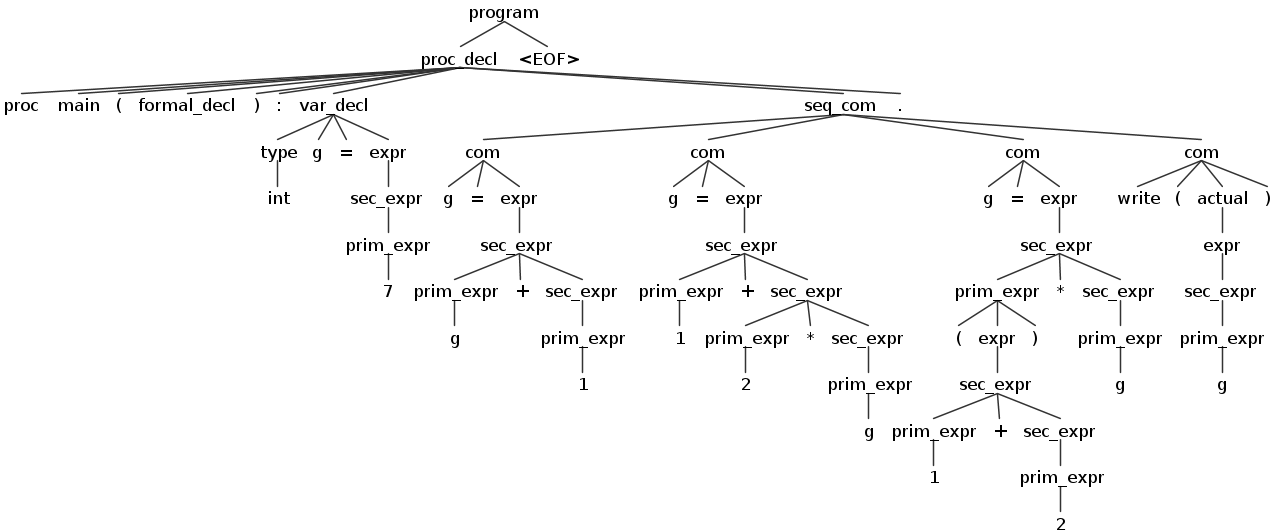
\includegraphics[height=5cm,width=\linewidth]{images/2-2a.png}
		\caption{Parse Tree/Concrete Syntax Tree}
		\label{fig:ANTLR-parse-tree}
	\end{subfigure}
	\begin{subfigure}[b]{0.5\textwidth}
		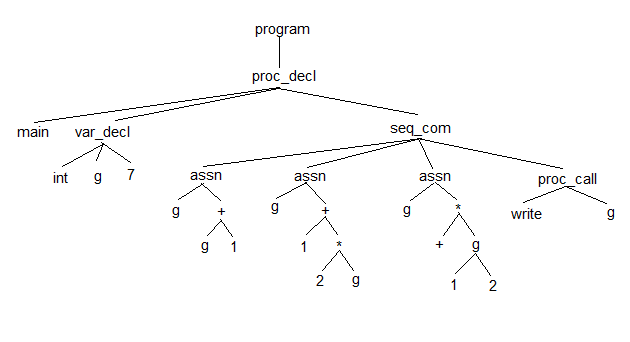
\includegraphics[height=5cm,width=\linewidth]{images/2-2b.png}
		\caption{Abstract Syntax Tree}
		\label{fig:ANTLR-syntax-tree}
	\end{subfigure}
	\caption{The ANTLR generated parse tree and the theoretical AST of the same Fun program}\label{fig:parse-abstract-tree}	
\end{figure}

Whilst this tool may serve to provide a preliminary understanding of how ANTLR forms a parse tree, we can immediately observe how large and difficult to read figure \ref{fig:ANTLR-parse-tree} is, in comparison to figure \ref{fig:ANTLR-syntax-tree}. There are many unnecessary tokens, such as EOFs, brackets and colons which serve only to obfuscate the diagram. The tree also contains many paths consisting of multiple unary branch nodes, which could easily be collapsed into a single edge.

Most of all, this tool provides nothing more than a simple diagram, it gives no indication of how this tree would be traversed during compilation, nor does it reveal any details of the internal workings of each node.

\chapter{Requirements}
\section{Methodology} 
After establishing that a product is worthwhile to build in the first place, most requirement elicitation approaches involve a repetitive cycle of expanding or reducing an initially small list of desiderata. After an initial interview with Simon Gay, the current lecturer of the {\it Programming Languages} course and proposer of this project, it was clear that whilst the project was inherently complex, the set of functional requirements was simple, well-defined and unlikely to change significantly in the future. For this reason, it was determined that extensive requirement gathering techniques, such as questionnaires or focus groups, were ultimately unnecessary; and all additional requirements were to be established through further interviews with Simon Gay.

\section{User Stories}
User stories are short and simple descriptions of a potential feature, told from the perspective of a potential user. User stories typically follow the template of:\\\\
\textit{As a \textbf{user type}, I want to \textbf{achieve some goal}, so that \textbf{justification.}}

User stories are a core component of the agile software development approach. They provide a means of considering the possible features that various different types of user may want in order to build a fuller set of functional requirements. User stories can also provide the basis for task estimation and prioritisation; however, since this project is not being developed by a team, these aspects won't be considered aside from a high-level prioritisation of end functional requirements.

\begin{itemize}
\item As a user, I want to read details about the Fun language, so that I can write valid Fun programs as input and better understand the compilation animations.
\item As a user, I want to be able to input any Fun program, so that I can learn about the compilation process in the general case, not just for specific examples.
\item As a user, I want to be able to view the animation of the contextual analysis phase of my program, so that I can understand how the compiler carries out this task.
\item As a user, I want to be able to view the animation of the code-generation phase of my program, so that I can understand how the compiler carries out this task.
\item As a user, I want to be able to play different sections of the compilation animation independently (i.e., contextual analysis or code generation), so that I can focus my learning on specific areas. 
\item As a user, I want to be able to replay an animation, so that I can review any details I missed/misunderstood.
\item As a user, I want to be able to step through the animation at my own pace, so I can easier understand what is happening during the animation.
\end{itemize}

\section{Functional Requirements}
After conducting several interviews with Simon Gay and analysing the above user stories, a formal list of functional requirements was created. Functional requirements are intended to capture a specific function of a system. The \textit {MoSCoW method} was used as a prioritisation technique for the following requirements. This method is another commonly used aspect of agile development, and involves partitioning requirements into four categories: \textit{Must have}, \textit{Should have}, \textit{Could have} or \textit{Would have}.
\subsection{Must Have}
\begin{itemize}
\item Allow users to view the AST for pre-defined Fun programs.
\begin{itemize}
\item At the very least, users should be able to choose from a small list of pre-written Fun programs and view the corresponding AST.
\end{itemize}
\end{itemize}
\subsection{Should Have}
\begin{itemize}
\item Allow users to view a simple continuous animation that demonstrates how the AST would be traversed during contextual analysis and code generation.
\begin{itemize}
\item The animation cannot be paused, reversed, or moved through step by step.
\end{itemize}
\item At the end of the animation, display some basic results of the compilation, including object code and address/type tables.
\begin{itemize}
\item These details would only be published at the end of the animation, not during.
\end{itemize}
\item Display information that explains how the Fun language works.
\begin{itemize}
\item This would involve effectively embedding the Fun specification somewhere within the application.
\end{itemize}
\end{itemize}
\subsection{Could Have}
\begin{itemize}
\item Allow users more control over the animation, including pausing, reversing, and step-wise movements - backwards and forwards.
\item Allow users to input any arbitrary Fun program and view the corresponding animation.
\begin{itemize}
\item The user is no longer restricted to using pre-defined example programs.
\end{itemize}
\item Display results of the animation as they occur during the compilation.
\begin{itemize}
\item For example, populate the type table as each variable is declared during the animation.
\end{itemize}
\item Display more in-depth analytical and informational details during the animation.
\begin{itemize}
\item This includes code templates and explanatory messages of the internal workings of each node as it is visited.
\end{itemize}
\end{itemize}
\subsection{Would Have}
\begin{itemize}
\item Execute and display the results of the generated object code.
\end{itemize}

\section{Non-functional Requirements}
In contrast to functional requirements that detail specific behaviours or a system, non-functional requirements measure an overall properties of a system. Non-functional requirements often consider areas such as security, usability and extensibility; overall utilities of a system.

\begin{itemize}
\item The application must work on all modern browsers.
\item The application must be able to interact efficiently with a Java-based application (the Fun compiler).
\item The application must be responsive, at least to a tablet level.
\item The application must ensure no malicious code can be executed.
\end{itemize}

%%%%%%%%%%%%%%%%
%              %
%  APPENDICES  %
%              %
%%%%%%%%%%%%%%%%
\begin{appendices}

\end{appendices}

%%%%%%%%%%%%%%%%%%%%
%   BIBLIOGRAPHY   %
%%%%%%%%%%%%%%%%%%%%

\bibliographystyle{plain}
%\bibliography{bib}

\end{document}
